\documentclass[border=10pt]{standalone}
\usepackage{pgfplots}
\pgfplotsset{compat=1.18}
\begin{document}
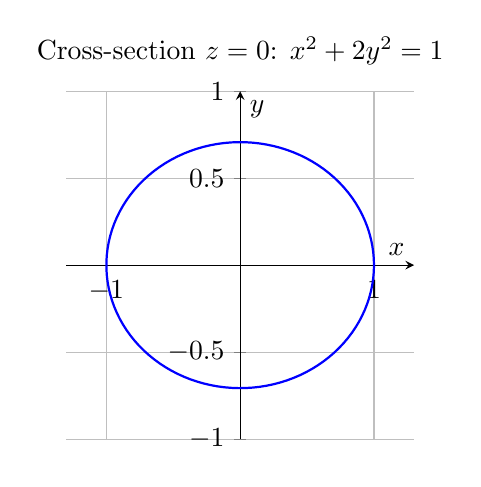
\begin{tikzpicture}
\begin{axis}[
    title={Cross-section $z=0$: $x^2 + 2y^2 = 1$},
    xlabel={$x$}, ylabel={$y$},
    xmin=-1.3, xmax=1.3, ymin=-1, ymax=1,
    axis lines=middle, grid=both, width=6cm, height=6cm,
]
\addplot[domain=0:360, samples=120, blue, thick] ({cos(x)}, {sin(x)/sqrt(2)});
\end{axis}
\end{tikzpicture}
\end{document}